\subsection{成果発表会}
\par
 ここでは成果発表会について述べる.
\par
  2014年12月12日に未来大にて前期と後期を通してのプロジェクト学習の成果を発表する成果発表会が行われた.それに向けて11月下旬から開発したアプリケーション「Cool Japanimation」と「Rhyth/Walk」の開発を進め,発表で使用するポスターとその補助である発表資料のスライドを作成した.
例年他大学のメンバと一緒に発表を行うが,諸事情があり,今回の最終発表会は未来大だけのメンバで行った.以下に成果発表会で用いた各種発表資料の準備内容と役割分担を示す.
\begin{enumerate}
\item 「Cool Japanimation」(HTML5班:全員,「Cool Japanimation」のAndroid班:全員)
\par
 「Cool Japanimation」はAndroidとiPhone端末で実装した.しかし,Androidでは実装が間に合わず,発表では実機を見せなかった.
 iPhoneではHTML5で実装し,2台実機を用意した.聴講者にはポスタの前でアニメ検索からツアー検索に遷移しツアー作成と参加の流れを主に説明しながら実機を動かし,成果を発表した.
\par
\item 「Rhyth/Walk」(「Rhyth/Walk」のAndroid班:全員,iOS班:全員)
\par
 「Rhyth/Walk」は機能のアルゴリズムの実装に時間がかかり,歩くテンポに合わせた選曲を行う機能を中心に実装した.
 Android端末では起動するとアプリケーションが落ちてしまい,動かせる状態ではなかった.iOS端末では1台用意されており,
 「Rhyth/Walk」は1台のみで聴講者にポスターの前で説明しながら実機を動かし,成果を発表した.


\item ポスター(未来大:中司,紺井,三栖)
\par
 成果発表会で使用するポスターは,中間発表会同様プロジェクトの概要を示したメインポスターを1枚,
 アプリケーションのそれぞれ説明を示したサブポスターを2枚,合計3枚作成した.成果発表会では,
 各アプリケーションのビジネスモデルの説明を加え,アプリケーションの流れを例を出し具体性のある内容にした.
 作成においては学生間や教員からの助言を参考に時間がある限り作り直した.発表会では聴衆から高い評価を得た.
 以下の図 9.2.3にそれぞれのポスターを示す.
\begin{center}
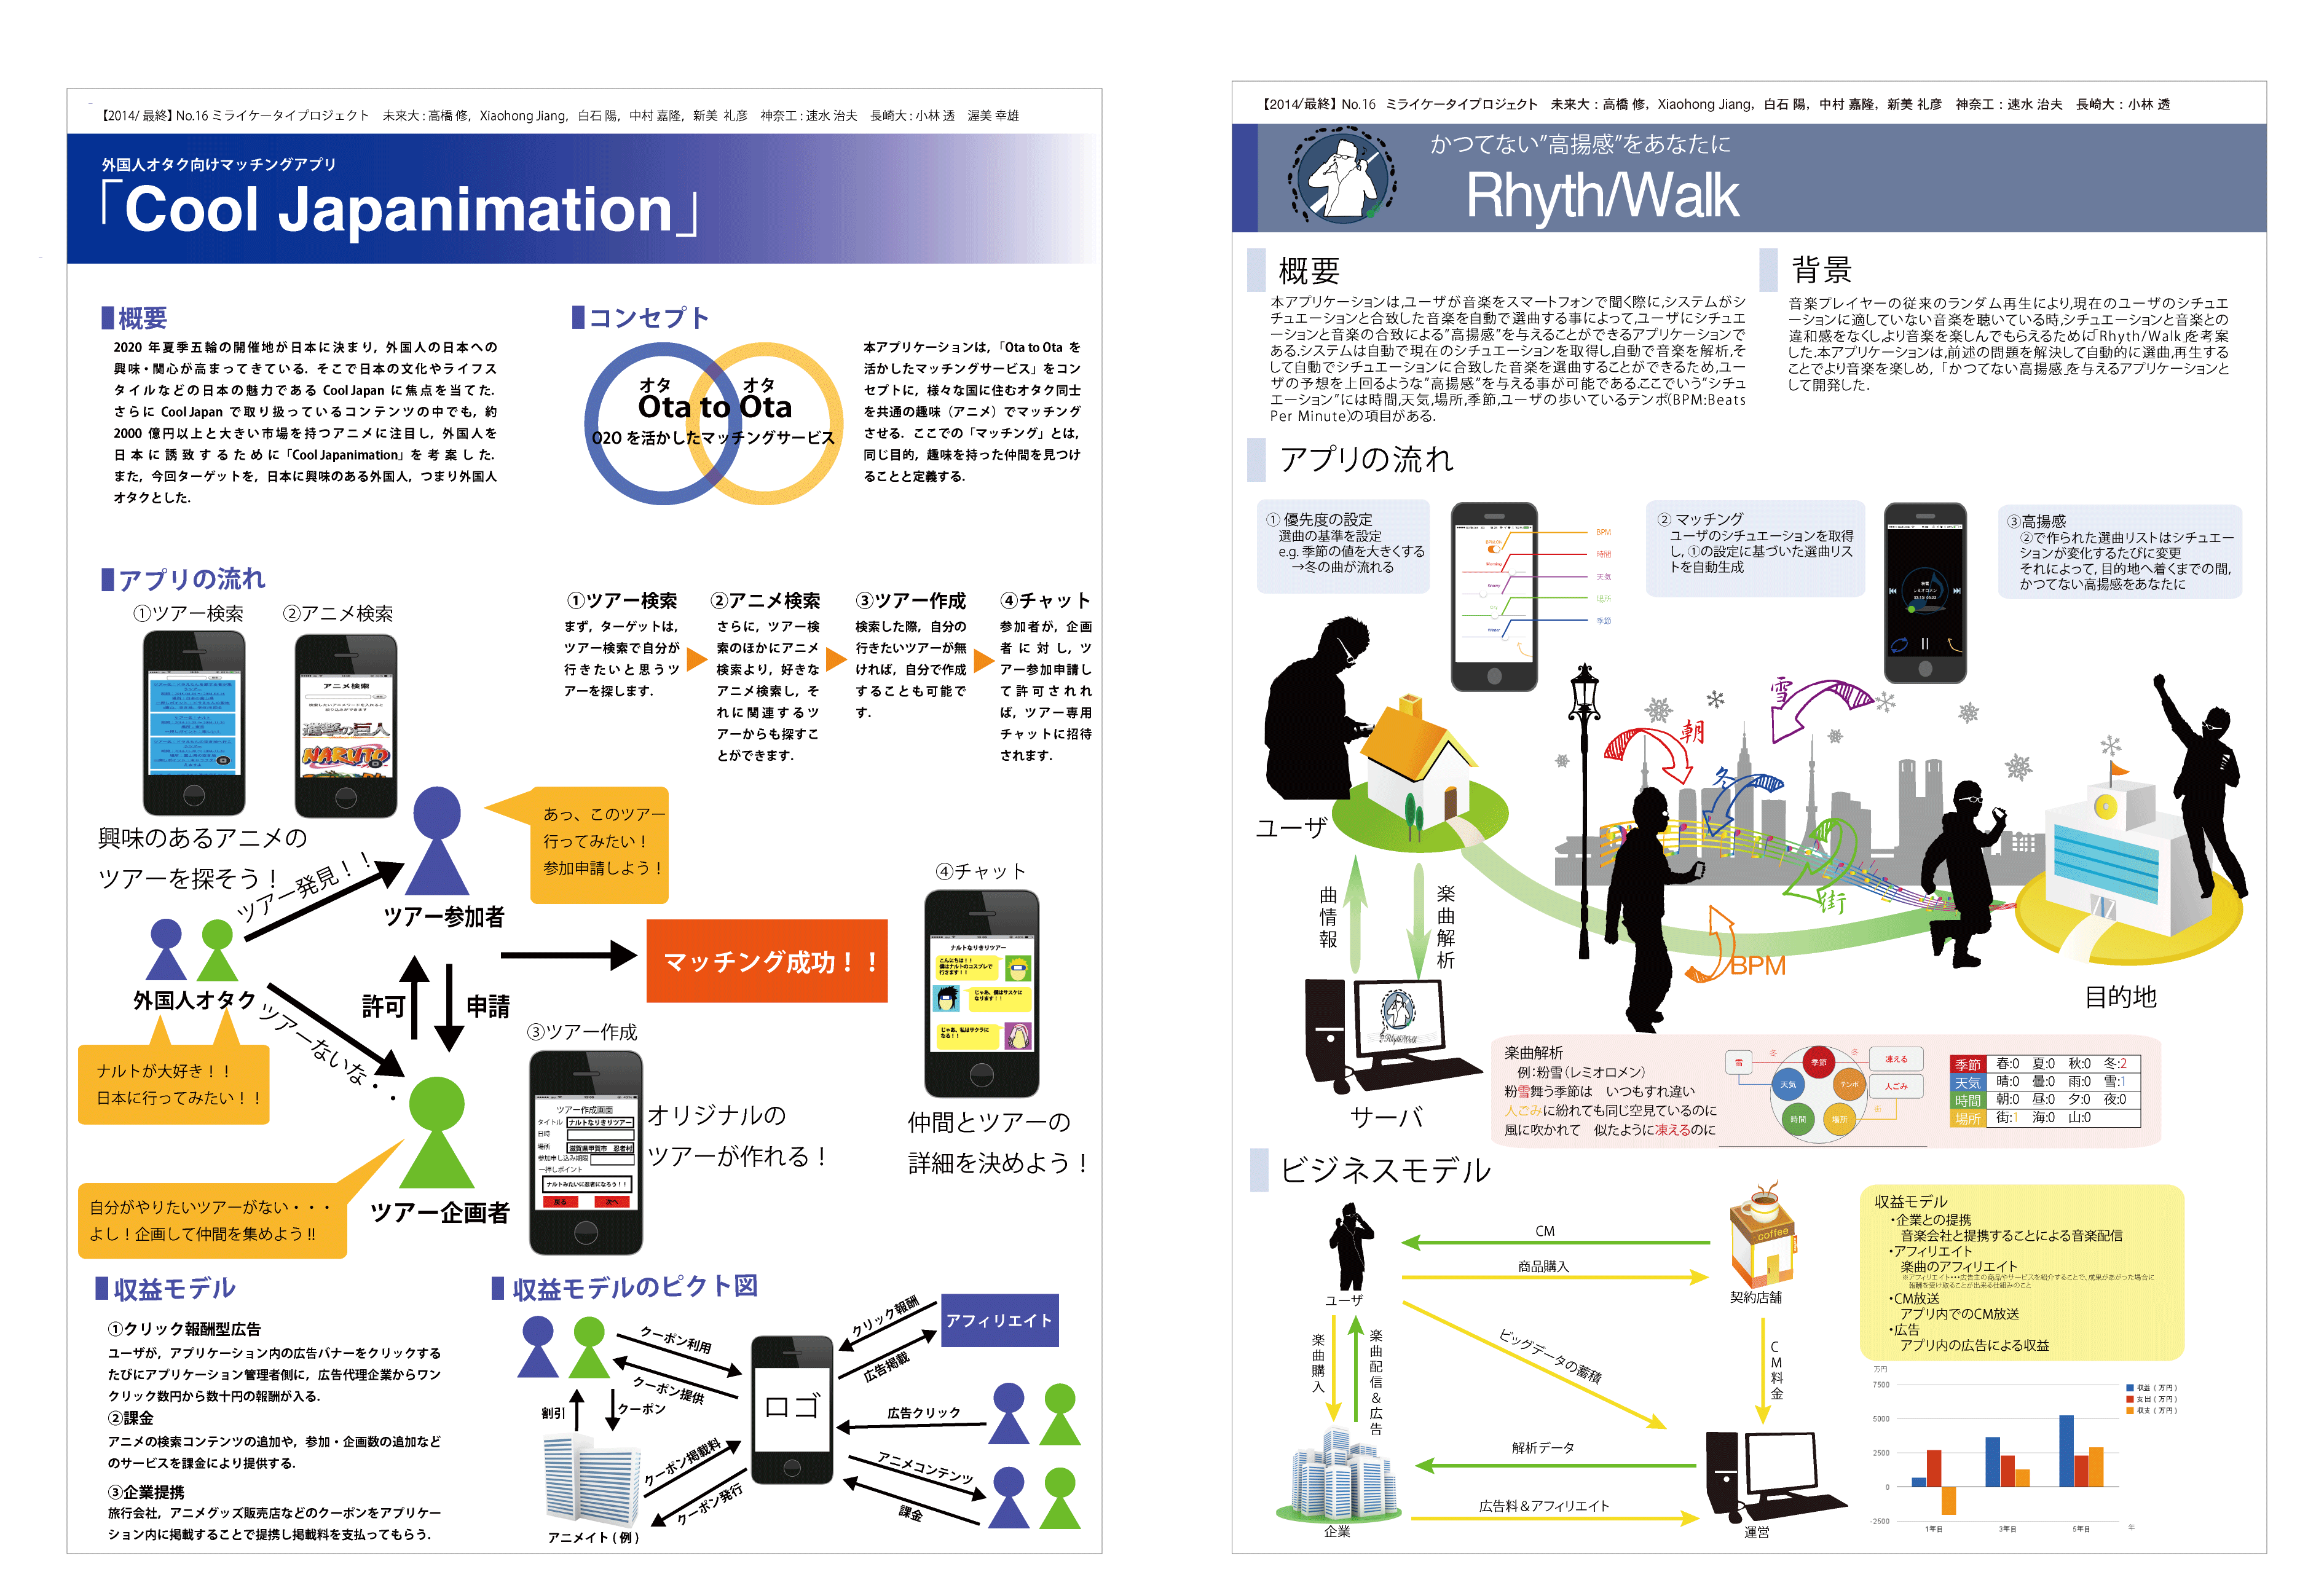
\includegraphics[width=10cm, bb=0 0 200 150]{poster.png} \\
  図 9.2.3: 成果発表ポスター(左:「Cool Japanimation」,右:「Rhyth/Walk」)
\end{center}

\item 発表用スライド(未来大:小笠原,藤原,鍋田)
\par
作成においては2月行われる提供企業先での発表を意識し作成した.また,中間発表会ではスライドのマージに
膨大に時間がかかったので解消すべく,編集人数を少なくし,スライドの拡張子をそろえるようにした.
「Cool Japanimation」に関して,プレゼンテーションは実装した画面を素材として使おうと試みたが,
テキストが小さく遠くから見えないので,スライド用に見やすい画像を再作成した.
「Rhyth/Walk」に関して,アプリのイメージを伝えるための動画を作成し、伝わりやすい発表を目指した.
中間発表会では各アプリの実装する予定段階の機能の説明を中心としたプレゼンテーションを行ったのだが、
成果発表会では各アプリの予定であった機能の実装した説明を中心としたので、
中間発表会と成果発表会との違いが分かりにくくなったプレゼンテーションになってしまった.
しかし、結果的に分かりやすかったと好評を得られた.

\item 発表者(未来大学生全員)
\par
作成されたスライド,ポスターを用いて聴講者の前で成果発表を行った.発表回数は6回で,メンバ12人が3人1組みで,6組で全員が発表を行った.スライドの内容を把握し,アドリブを加えながら発表者それぞれの言葉で行った.成果発表会直前にプレゼンテーションをメンバで相互レビューし合うなど発表練習を綿密に行った.当日は多くの来場者に本プロジェクトの活動と成果を伝えることができた.
\item 評価シート(未来大:藤原)
\par
評価シートは全体を通しての発表技術と内容,各アプリケーションケーションの魅力とについての評価を10段階評価と自由記入欄を設けた.
評価シートは WG のテンプレートではアプリケーションについての評価を得ることができなかったので,
裏面にアプリケーションについて評価していただけるように新しくそれぞれのコメント欄を設けた.
評価シートの内容は"発表技術", "発表内容", "「Cool Japanimation」", "「Rhyth/Walk」"についてと 10 段階で評価してもらい,
それぞれの評価基準は"プロジェクトの内容を伝えるために,効果的な発表が行われているか", 
"プロジェクトの目標設定と計画は十分なものであるか", アプリケーションそれぞれに"使いたいと思えるアプリケーションだったか"
とした.また点数だけでなくアドバイスや意見を多く書けるように"このアプリケーションについてアドバイス等ありましたら
記入をお願いします"のコメント欄をとった.なお 10 段階評価は 1 が悪く 10 が良いとなっている.
評価シートと他に1 から 6 までの番号をあらかじめ記入した紙を用意し, 回収したらその紙に挟むことで,
どの発表者の評価なのかわかるようにした.集計した評価シートは 83 枚となった.全体の平均点は"発表技術", "発表内容", 
"「Cool Japanimation」", "「Rhyth/Walk」"の順に 7.83,7.87,7.08,7.54 となった.コメントとしては,"発表技術"
については,声が大きく聞き取りやすかった,スライドが見やすかった,というコメントが多かった."発表内容"
については,アプリが具体的で分かりやすかった,面白そうというコメントが多かった.「Cool Japanimation」については,
SNSとの違いが分からない,ターゲットの規模が大きすぎて漠然としている,マッチングの意味がよくわかならい,というコメントが多く,
発表では伝えきれていない部分が多かった.「Rhyth/Walk」については,シチュエーションにあった音楽が聞けるのは面白そうだけど,
もう一捻り欲しい,ユーザの喜怒哀楽を反映してほしい,というコメントが多く,これからの展望に期待しているコメントが多かった.
これらコメントはアドバイスが多く,これを参考に今後の改善を行う.


\end{enumerate} 
\par
全体評価
\par 評価内容を踏まえて自分のグループの評価を目的,現状の把握,今後の計画の具体性,表現力,
チームワーク,をもとに自分たちの発表を 10 段階で客観的に評価すると,10と評価する.評価理由としては,
プロジェクト自体の目的,現状の把握,アプリケーションの魅力ともに, 十分に表現することができ,
プロジェクトのイメージが伝わった,アプリケーションを使ってみたいといった意見を頂いたからである.
プロジェクトのイメージを聴講者に疑問を抱かせることがなく,ミライケータイプロジェクトのイメージを伝えることができた.
表現力に関してはスライドのデザイン,声量,質疑応答ともに良い意見を頂いた.チームワークの面でも,ポスター,スライドともに,担当者が責任を持って作成を行ない最後まであきらめず,それに対するレビューもOB・OGを含めプロジェクトメンバ一丸となり, 取り組む事ができた.

\bunseki{中司 智朱希(未来大)}
